

\tikzset{every picture/.style={line width=0.75pt}} %set default line width to 0.75pt        

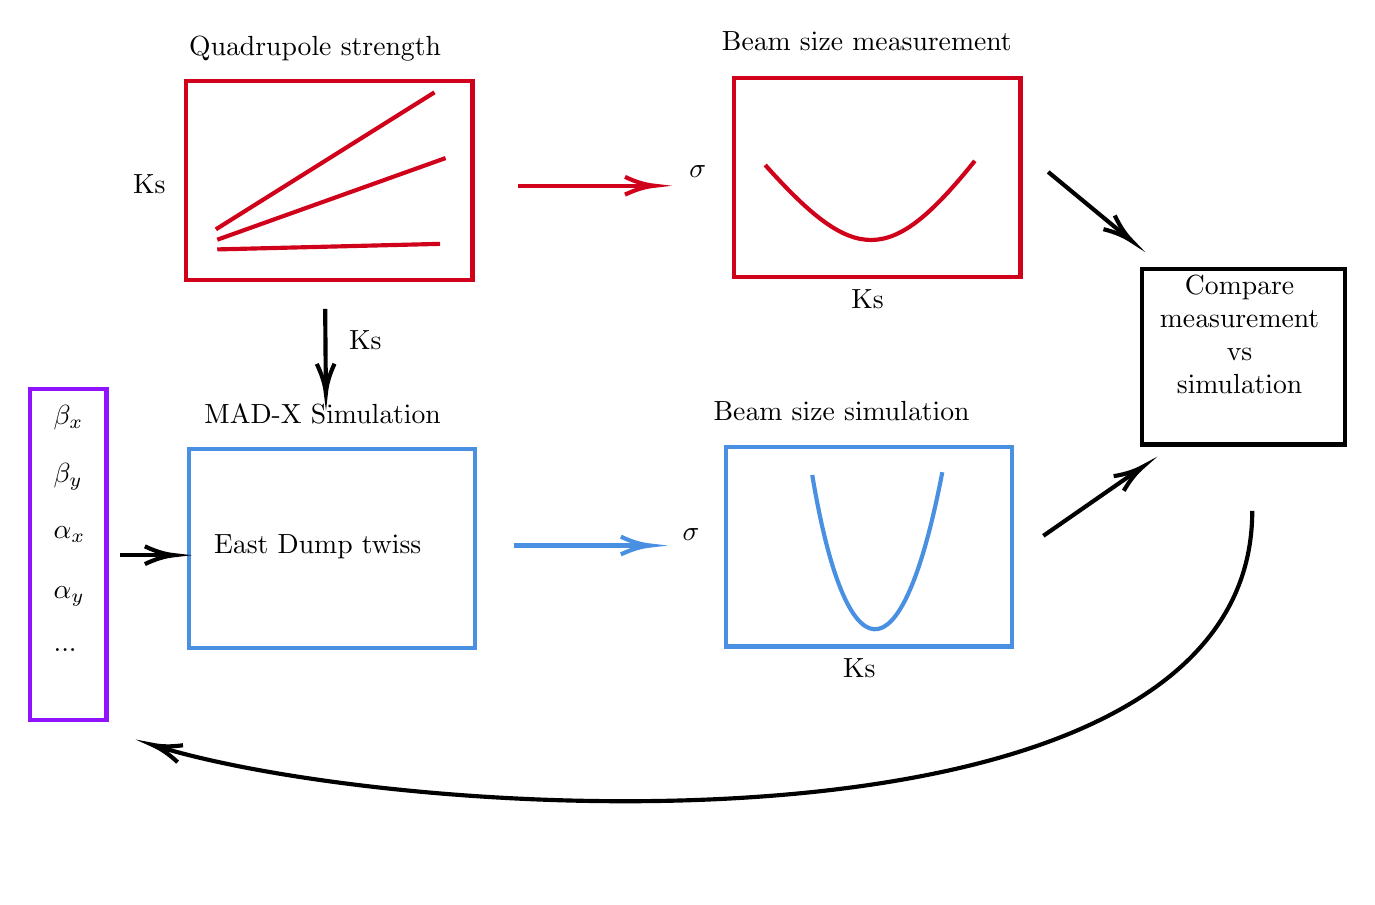
\begin{tikzpicture}[x=0.75pt,y=0.75pt,yscale=-1,xscale=1]
%uncomment if require: \path (0,480); %set diagram left start at 0, and has height of 480

%Shape: Rectangle [id:dp4246347329167801] 
\draw  [color={rgb, 255:red, 208; green, 2; blue, 27 }  ,draw opacity=1 ][line width=1.5]  (362.67,99.33) -- (500.67,99.33) -- (500.67,195.33) -- (362.67,195.33) -- cycle ;
%Curve Lines [id:da9888709896390471] 
\draw [color={rgb, 255:red, 208; green, 2; blue, 27 }  ,draw opacity=1 ][line width=1.5]    (377.67,141.33) .. controls (420.67,189.33) and (437.67,190.33) .. (478.67,139.33) ;
%Shape: Rectangle [id:dp49952149002749646] 
\draw  [color={rgb, 255:red, 208; green, 2; blue, 27 }  ,draw opacity=1 ][line width=1.5]  (98.67,100.67) -- (236.67,100.67) -- (236.67,196.67) -- (98.67,196.67) -- cycle ;
%Straight Lines [id:da9425896029593615] 
\draw [color={rgb, 255:red, 208; green, 2; blue, 27 }  ,draw opacity=1 ][line width=1.5]    (113,172.33) -- (218.33,106.33) ;
%Straight Lines [id:da0776144392613658] 
\draw [color={rgb, 255:red, 208; green, 2; blue, 27 }  ,draw opacity=1 ][line width=1.5]    (113.67,177.33) -- (223.67,138) ;
%Straight Lines [id:da02037742317127811] 
\draw [color={rgb, 255:red, 208; green, 2; blue, 27 }  ,draw opacity=1 ][line width=1.5]    (113.67,182) -- (221,179.33) ;
%Straight Lines [id:da070053405995959] 
\draw [color={rgb, 255:red, 208; green, 2; blue, 27 }  ,draw opacity=1 ][line width=1.5]    (258.67,151.33) -- (321.33,151.33) ;
\draw [shift={(324.33,151.33)}, rotate = 180] [color={rgb, 255:red, 208; green, 2; blue, 27 }  ,draw opacity=1 ][line width=1.5]    (14.21,-4.28) .. controls (9.04,-1.82) and (4.3,-0.39) .. (0,0) .. controls (4.3,0.39) and (9.04,1.82) .. (14.21,4.28)   ;
%Shape: Rectangle [id:dp944364271889234] 
\draw  [color={rgb, 255:red, 144; green, 19; blue, 254 }  ,draw opacity=1 ][line width=1.5]  (23.33,249.33) -- (60.33,249.33) -- (60.33,408.67) -- (23.33,408.67) -- cycle ;
%Straight Lines [id:da8395245156263087] 
\draw [color={rgb, 255:red, 0; green, 0; blue, 0 }  ,draw opacity=1 ][line width=1.5]    (165.67,210.67) -- (165.98,248.33) ;
\draw [shift={(166,251.33)}, rotate = 269.53] [color={rgb, 255:red, 0; green, 0; blue, 0 }  ,draw opacity=1 ][line width=1.5]    (14.21,-4.28) .. controls (9.04,-1.82) and (4.3,-0.39) .. (0,0) .. controls (4.3,0.39) and (9.04,1.82) .. (14.21,4.28)   ;
%Shape: Rectangle [id:dp4855606702968256] 
\draw  [color={rgb, 255:red, 74; green, 144; blue, 226 }  ,draw opacity=1 ][line width=1.5]  (100,278) -- (238,278) -- (238,374) -- (100,374) -- cycle ;
%Straight Lines [id:da7022632349262303] 
\draw [line width=1.5]    (66.67,329.33) -- (90,329.33) ;
\draw [shift={(93,329.33)}, rotate = 180] [color={rgb, 255:red, 0; green, 0; blue, 0 }  ][line width=1.5]    (14.21,-4.28) .. controls (9.04,-1.82) and (4.3,-0.39) .. (0,0) .. controls (4.3,0.39) and (9.04,1.82) .. (14.21,4.28)   ;
%Straight Lines [id:da3968621494939437] 
\draw [color={rgb, 255:red, 74; green, 144; blue, 226 }  ,draw opacity=1 ][line width=1.5]    (256.67,324.67) -- (319.33,324.67) ;
\draw [shift={(322.33,324.67)}, rotate = 180] [color={rgb, 255:red, 74; green, 144; blue, 226 }  ,draw opacity=1 ][line width=1.5]    (14.21,-4.28) .. controls (9.04,-1.82) and (4.3,-0.39) .. (0,0) .. controls (4.3,0.39) and (9.04,1.82) .. (14.21,4.28)   ;
%Shape: Rectangle [id:dp4118518001915987] 
\draw  [color={rgb, 255:red, 74; green, 144; blue, 226 }  ,draw opacity=1 ][line width=1.5]  (358.67,277.33) -- (496.67,277.33) -- (496.67,373.33) -- (358.67,373.33) -- cycle ;
%Curve Lines [id:da2553267141266382] 
\draw [color={rgb, 255:red, 74; green, 144; blue, 226 }  ,draw opacity=1 ][line width=1.5]    (400.33,290.67) .. controls (416.33,386.67) and (443,393.33) .. (463,289.33) ;
%Shape: Rectangle [id:dp8890861260646525] 
\draw  [line width=1.5]  (559.33,191.33) -- (657,191.33) -- (657,276) -- (559.33,276) -- cycle ;
%Curve Lines [id:da18599849782409872] 
\draw [line width=1.5]    (612.33,308) .. controls (612.33,483.12) and (203.78,458.25) .. (84.12,421.23) ;
\draw [shift={(82.33,420.67)}, rotate = 17.65] [color={rgb, 255:red, 0; green, 0; blue, 0 }  ][line width=1.5]    (14.21,-4.28) .. controls (9.04,-1.82) and (4.3,-0.39) .. (0,0) .. controls (4.3,0.39) and (9.04,1.82) .. (14.21,4.28)   ;
%Straight Lines [id:da014820791284121837] 
\draw [line width=1.5]    (511.67,320) -- (557.2,288.38) ;
\draw [shift={(559.67,286.67)}, rotate = 145.22] [color={rgb, 255:red, 0; green, 0; blue, 0 }  ][line width=1.5]    (14.21,-4.28) .. controls (9.04,-1.82) and (4.3,-0.39) .. (0,0) .. controls (4.3,0.39) and (9.04,1.82) .. (14.21,4.28)   ;
%Straight Lines [id:da7493093229877397] 
\draw [line width=1.5]    (514,144.67) -- (552.02,176.09) ;
\draw [shift={(554.33,178)}, rotate = 219.57] [color={rgb, 255:red, 0; green, 0; blue, 0 }  ][line width=1.5]    (14.21,-4.28) .. controls (9.04,-1.82) and (4.3,-0.39) .. (0,0) .. controls (4.3,0.39) and (9.04,1.82) .. (14.21,4.28)   ;

% Text Node
\draw (417.67,199.83) node [anchor=north west][inner sep=0.75pt]   [align=left] {Ks};
% Text Node
\draw (339.67,140.33) node [anchor=north west][inner sep=0.75pt]   [align=left] {$\displaystyle \sigma $};
% Text Node
\draw (71.67,144.5) node [anchor=north west][inner sep=0.75pt]   [align=left] {Ks};
% Text Node
\draw (98.67,77.67) node [anchor=north west][inner sep=0.75pt]   [align=left] {Quadrupole strength};
% Text Node
\draw (355.33,75.67) node [anchor=north west][inner sep=0.75pt]   [align=left] {Beam size measurement};
% Text Node
\draw (33.33,255.4) node [anchor=north west][inner sep=0.75pt]    {$\beta _{x}$};
% Text Node
\draw (33.33,283.4) node [anchor=north west][inner sep=0.75pt]    {$\beta _{y}$};
% Text Node
\draw (33.33,314.07) node [anchor=north west][inner sep=0.75pt]    {$\alpha _{x}$};
% Text Node
\draw (33.33,342.73) node [anchor=north west][inner sep=0.75pt]    {$\alpha _{y}$};
% Text Node
\draw (33.33,372.73) node [anchor=north west][inner sep=0.75pt]    {$...$};
% Text Node
\draw (106,255) node [anchor=north west][inner sep=0.75pt]   [align=left] {MAD-X Simulation};
% Text Node
\draw (110.67,317.67) node [anchor=north west][inner sep=0.75pt]   [align=left] {East Dump twiss};
% Text Node
\draw (413.67,377.83) node [anchor=north west][inner sep=0.75pt]   [align=left] {Ks};
% Text Node
\draw (336.33,315) node [anchor=north west][inner sep=0.75pt]   [align=left] {$\displaystyle \sigma $};
% Text Node
\draw (351.33,253.67) node [anchor=north west][inner sep=0.75pt]   [align=left] {Beam size simulation};
% Text Node
\draw (561.33,193) node [anchor=north west][inner sep=0.75pt]   [align=left] {\begin{minipage}[lt]{65.09pt}\setlength\topsep{0pt}
\begin{center}
Compare\\measurement\\vs\\simulation
\end{center}

\end{minipage}};
% Text Node
\draw (175.67,219.83) node [anchor=north west][inner sep=0.75pt]   [align=left] {Ks};

\end{tikzpicture}
